\chapter{Introduction}
\label{c:intro}

\section{Motivation}
<<<<<<< HEAD
Since the cost of existing software solution is too high, and has little flexibility while tunning algorithms.
The

\subsection{Previous Solution}
add previous work here.



\section{Related Works}
\label{section:related-work}
add referenced paper here and write some comment

\section{Goal}
\label{section:goal}
Design a system that is both cost efficient and time efficient. Could identify lettering defect and LED light defect on keyboard.
=======
\label{section:motivation}
High-tech tools are prevalent nowadays and many of our daily are now routinely performed with computers. People write articles with computers; people draw diagrams with computers; people, of course, design programs with computers. Among our various usages of computers, one of them is music composition. For the purpose of storing and visualizing musicians' creation, the standard western musical score, which contains information pertaining to how a piece of music should be played, has been used for hundreds of years and around the globe. However, the score was designed for human beings instead of computers, and most of scores are scanned and stored as images, which means nothing but lots of pixels for computers. In other words, these scores are not yet symbolically represented. Therefore, the concern of this dissertation is \emph{optical music recognition} (OMR), which refers to the development of methods that automatically convert score images into their symbolic representation.

\section{Goal}
\label{section:goal}
Design a software that converts a score image (.png / .jpeg / .bmp / .pdf) into its symbolic representation encoded in a format that is readable by a computer such as MusicXML.
>>>>>>> parent of 2a4e8fe... updated

\section{Divide and Conquer}
% \subsection{Definition}
% \label{section:divide-and-conquer}

% Fig.~\ref{fig:DnC} shows the concepts of \emph{divide and conquer} (D\&C). D\&C is an algorithm design paradigm that breaks a complex problem into a couple of relatively simple subproblems, to \emph{divide}, then solves them respectively, to \emph{conquer}. Before conquering, the problem will be divided recursively until it is simple enough to be processed. Finally, the solutions to the subproblems will be merged as those to the original problem.

% \begin{figure}[!htb]
%     \centering
%     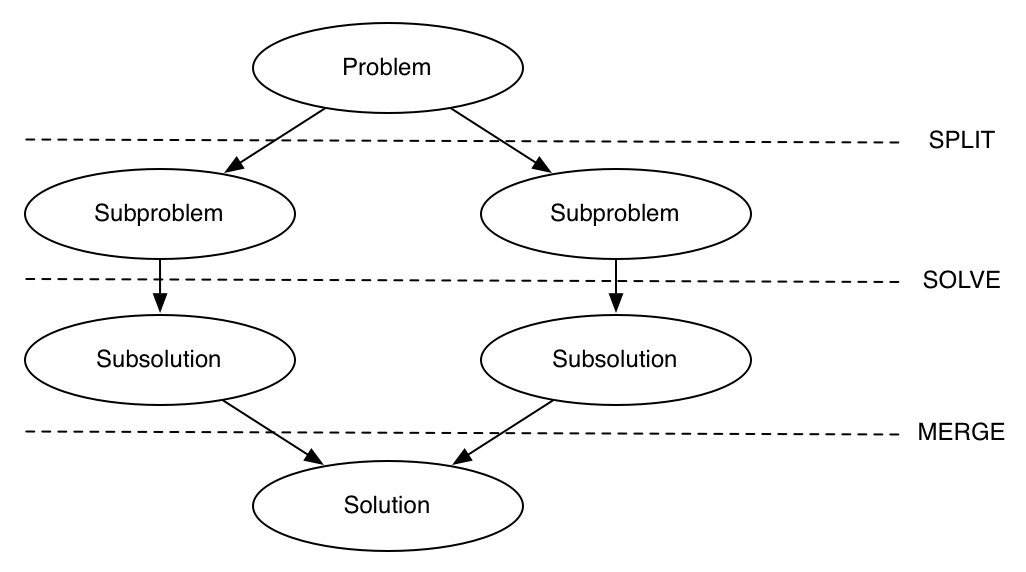
\includegraphics[width=\textwidth]{figsrc/DnC.png}
%     \caption{A diagram showing how divide and conquer works.\label{fig:DnC}}
% \end{figure}

\subsection{Main Contribution of This Dissertation}
\label{subsec:advantages}

\subsubsection{Reducing the Difficulty of Problems}

\subsubsection{Independence of Subproblems}

\subsubsection{Parallelism}


% Nowadays, a processor usually has multiple cores, and lots of computational tasks are implemented to be executed with parallel programs. In D\&C algorithm, the functions solving split subproblems are identically designed. With high independence and similar operations between subproblems, it is a good strategy to process them simultaneously. In other word, the original problem is suitable to be solved with \emph{SIMD (Single-Instruction-Multiple-Data)} parallel programs.
